% Replacement text for the Methodology, Results, and Discussion portions of
% the AAAI manuscript.  This version is designed for the eight-page body:
% two compact tables and four figures replace the current longtable block.
%
% MBR is the manuscript abbreviation for the Kaggle malware/benign collection
% published by Aashish.zzz.  The historical BibTeX key `synthetic` is retained
% below so that this file works with the bibliography used in the current
% draft; the source itself is not described as synthetic.

\section{Methodology}

\subsection{Study Design}

We conducted a controlled comparison of exact, simulated, and hardware-measured quantum kernels for binary malware classification. The experiment comprised six dataset--representation configurations, three repeated held-out splits per configuration, and four quantum execution environments. CLaMP and the Malware and Benign Recognition (MBR) data were evaluated in both a selected native representation and a four-component principal-component representation; CIC-YNU-IoTMal and EMBER2018 were evaluated with four components because their original feature spaces exceeded the hardware widths used in this study. MBR is the abbreviation used here for the Kaggle malware/benign collection published by Aashish.zzz~\cite{synthetic}; it replaces the preliminary internal label ``Fabiana.'' Frozen artifact identifiers retain the prefix \texttt{fabiana\_} so that completed runs remain traceable.

\begin{table*}[t]
\centering
\small
\caption{Datasets and evaluated representations. Candidate-pool counts are after deterministic source sampling, where applicable, and removal of duplicate feature vectors. Labels 0 and 1 denote benign and malware, respectively.}
\label{tab:dataset-design}
\begin{tabular}{lp{2.75in}rrl}
\toprule
Dataset & Observation and predictors & Source rows & Candidate pool & Configuration(s) \\
\midrule
CLaMP & Windows PE file; 10 selected header fields & 5,184 & 4,040 & Native-10, PCA-4 \\
MBR & Windows PE file; 8 selected header fields & 1,156 & 895 & Native-8, PCA-4 \\
CIC-YNU-IoTMal & Sandbox system-activity record; 314 numeric SAR fields & 2,121,949 & 1,280 & PCA-4 \\
EMBER2018 & Windows PE file; 2,381-dimensional static feature vector & 799,912 & 1,200 & PCA-4 \\
\bottomrule
\end{tabular}
\end{table*}

\subsection{Datasets and Predictors}

CLaMP~\cite{clamp} contains static Windows Portable Executable (PE) metadata. We selected \texttt{NumberOfSections}, \texttt{Characteristics}, \texttt{Magic}, \texttt{MajorLinkerVersion}, \texttt{SizeOfCode}, \texttt{AddressOfEntryPoint}, \texttt{ImageBase}, \texttt{SizeOfImage}, \texttt{DllCharacteristics}, and \texttt{SizeOfStackReserve}. The 5,184 source rows produced 4,040 unique, consistently labeled feature vectors: 2,275 benign and 1,765 malware. Duplicate filtering removed 1,144 rows and found no identical vector with conflicting labels.

MBR uses static PE metadata from the Kaggle collection cited above. We selected \texttt{SizeOfCode}, \texttt{SizeOfInitializedData}, \texttt{SizeOfUninitializedData}, \texttt{AddressOfEntryPoint}, \texttt{BaseOfData}, \texttt{ImageBase}, \texttt{NumberOfSections}, and \texttt{DllCharacteristics}. Its 1,156 rows produced 895 unique, consistently labeled vectors: 546 benign and 349 malware. Filtering removed 261 duplicates and found no conflicting-label vector.

CIC-YNU-IoTMal 2026~\cite{cic} contains Linux system-activity reports collected while benign and malicious IoT binaries ran in sandboxes for ARM, MIPS, MIPSEL, and x86. The 314 numeric fields shared by the four architecture files cover processor use, processes and context switches, interrupts, paging and swap, memory, storage, network, and file-system activity. Every row whose \texttt{MalwareFamily} value was not \texttt{Benign} received label 1. From 2,121,949 source rows, we deterministically sampled 160 benign and 160 malicious candidates per architecture, giving 1,280 rows balanced by class and architecture.

EMBER2018~\cite{ember2018} represents Windows PE files through 2,381 static features derived from byte and byte-entropy histograms, strings, general and header metadata, sections, imports, exports, and data directories. From the local 799,912-row vectorized release, we excluded unlabeled rows and deterministically selected 600 rows from each of labels 0 and 1. Neither CIC nor the sampled EMBER candidate pool contained duplicate full feature vectors or conflicting-label vectors.

For each dataset, full feature vectors were hashed before splitting. Identical vectors with one label were represented once; groups containing both labels were excluded. Source-row identifiers, feature hashes, source-file hashes, labels, and all selected indices were retained in the artifact.

\subsection{Splitting and Preprocessing}

We generated three deterministic repeated holdouts using master seed 20,260,825 and split-specific training seeds 101, 204, and 303. Each split contained 80 training and 80 test observations, with 40 benign and 40 malware observations in each partition. The three test sets were source-row disjoint and were reserved before any training draw; no training set contained a row assigned to any test set. Training sets could overlap across splits. CIC partitions additionally contained 10 observations from each class--architecture stratum. CLaMP native/PCA and MBR native/PCA conditions used identical row identifiers and labels within each split.

All transformations were fitted only to the corresponding 80-row training partition. Missing and infinite values were replaced through median imputation. Native inputs were then min--max scaled to $[0,1]$. PCA inputs were standardized, transformed with full-SVD PCA to four components, and min--max scaled to $[0,1]$; out-of-range test coordinates were clipped. The mean cumulative training variance represented by four components was 0.671 for CLaMP, 0.850 for MBR, 0.529 for CIC, and 0.343 for EMBER2018. Every transformed matrix was checked for finite values, and no test vector exactly matched a transformed training vector.

\subsection{Quantum Kernel and Execution Environments}

Each input coordinate was assigned to one qubit. We used Qiskit's \texttt{zz\_feature\_map} with two repetitions and linear entanglement~\cite{qiskit2024}. For feature-map unitary $U_{\phi}$, the kernel was
\begin{equation}
K(\mathbf{x},\mathbf{z})=
\left|\langle 0^{d}|U_{\phi}^{\dagger}(\mathbf{z})
U_{\phi}(\mathbf{x})|0^{d}\rangle\right|^{2},
\label{eq:fidelity-kernel}
\end{equation}
with $d\in\{4,8,10\}$. We evaluated four environments: (1) exact statevector fidelity; (2) an ideal Aer simulation of the transpiled circuit with 512 shots; (3) Aer with 512 shots and a noise model constructed from the IBM backend-property snapshot; and (4) 512-shot execution on \texttt{ibm\_rensselaer}. The ideal, noisy, and hardware conditions used the same transpiled instruction-set circuit. Active physical wires and their noise channels were relabeled densely for Aer without altering circuit operations.

The fidelity circuit applied $U_{\phi}(\mathbf{x})$, followed by $U_{\phi}^{\dagger}(\mathbf{z})$, measured every qubit, and estimated the kernel entry as the all-zero outcome frequency. For each condition, the symmetric training kernel required $80(79)/2=3,160$ off-diagonal evaluations; its diagonal was fixed to one. The test kernel required $80\times80=6,400$ evaluations. Thus each shot-based condition comprised 9,560 circuit evaluations and 4,894,720 shots.

Circuits were transpiled once for the target backend at optimization level 3 with transpiler seed 42. The resulting 4-, 8-, and 10-qubit circuits had depths 98, 170, and 206; total gate counts 174, 400, and 518; CZ counts 22, 54, and 70; and estimated durations 5.308, 7.524, and 8.660 $\mu$s, respectively. Dynamical decoupling, gate twirling, measurement twirling, and measurement-error mitigation were disabled. The hardware campaign used \texttt{ibm\_rensselaer} on August 26, 2026, from an initial backend snapshot dated August 25, 2026. All 18 primary jobs and three prespecified split-zero repeat jobs completed without failure or resubmission.

\subsection{Classification, Baselines, and Analysis}

Finite-shot training kernels were symmetrized, assigned a unit diagonal, and projected onto the positive-semidefinite cone by eigendecomposition and clipping negative eigenvalues to zero. The reconstructed matrix was normalized to unit diagonal. The same procedure was applied to exact training kernels; rectangular test kernels were not projected. A support-vector classifier (SVC) with a precomputed kernel and fixed $C=1$ was then fitted to each training kernel. Matched classical checks used linear and radial-basis-function (RBF) SVCs with $C=1$ and, for RBF, \texttt{gamma=scale}. These models received the same transformed inputs as the quantum method. No model or preprocessing hyperparameter was selected from test or hardware results.

The primary endpoint was balanced accuracy; ROC AUC from SVC decision scores was secondary. Kernel distortion relative to the exact test kernel was measured by relative Frobenius error,
$\|K_m-K_e\|_F/\|K_e\|_F$, and Pearson correlation between flattened kernel entries. Reported means and standard deviations are across the three held-out splits. We formed 95\% intervals from 10,000 bootstrap replicates by resampling rows separately within each split and class and averaging the split metrics. Six hardware-versus-exact prediction comparisons and two native-versus-PCA hardware comparisons used exact McNemar tests on the 240 paired held-out predictions; Holm's method controlled familywise error across the eight prespecified contrasts~\cite{mcnemar1947,holm1979}. Three-split compression intervals and correlations with circuit resources were treated as descriptive. The implementation used Python 3.12.3, Qiskit 2.5.1, Aer 0.17.2, Qiskit Machine Learning 0.9.0, Qiskit IBM Runtime 0.48.0, and scikit-learn 1.9.0.

\section{Results}

\subsection{Predictive Performance Across Environments}

Table~\ref{tab:primary-results} reports the exact and hardware endpoints, and Figure~\ref{fig:execution-performance} includes the two Aer conditions. Mean hardware-minus-exact balanced-accuracy changes ranged from $-1.67$ to $+1.25$ percentage points. The changes were $+0.42$ points for CLaMP native-10, $-0.42$ for CLaMP PCA-4, $-1.67$ for MBR native-8, $-0.83$ for MBR PCA-4, $+1.25$ for CIC PCA-4, and $-0.42$ for EMBER2018 PCA-4. None of the six hardware-versus-exact McNemar comparisons was significant after Holm adjustment; every adjusted $p$-value was 1.0. Across these comparisons, only 2--19 of 240 paired predictions were discordant.

\begin{table*}[t]
\centering
\small
\caption{Primary exact and IBM hardware results. BA is balanced accuracy, intervals are 95\% class-stratified bootstrap intervals, $\Delta$ is hardware minus exact in percentage points, AUC is reported as exact/hardware, and hardware kernel error and correlation are relative to the exact test kernel.}
\label{tab:primary-results}
\begin{tabular}{lccrccc}
\toprule
Configuration & Exact BA [95\% CI] & Hardware BA [95\% CI] & $\Delta$ & AUC E/H & HW error & HW corr. \\
\midrule
CLaMP native-10 & .842 [.796, .883] & .846 [.800, .888] & +0.4 & .926/.915 & .479 & .970 \\
CLaMP PCA-4 & .750 [.696, .804] & .746 [.692, .800] & $-0.4$ & .839/.817 & .112 & .996 \\
MBR native-8 & .975 [.954, .992] & .958 [.933, .979] & $-1.7$ & .982/.980 & .441 & .924 \\
MBR PCA-4 & .938 [.904, .967] & .929 [.896, .958] & $-0.8$ & .963/.961 & .114 & .997 \\
CIC PCA-4 & .692 [.633, .746] & .704 [.646, .758] & +1.3 & .780/.777 & .111 & .997 \\
EMBER2018 PCA-4 & .617 [.558, .671] & .613 [.558, .667] & $-0.4$ & .741/.723 & .111 & .997 \\
\bottomrule
\end{tabular}
\end{table*}

\begin{figure*}[t]
  \centering
  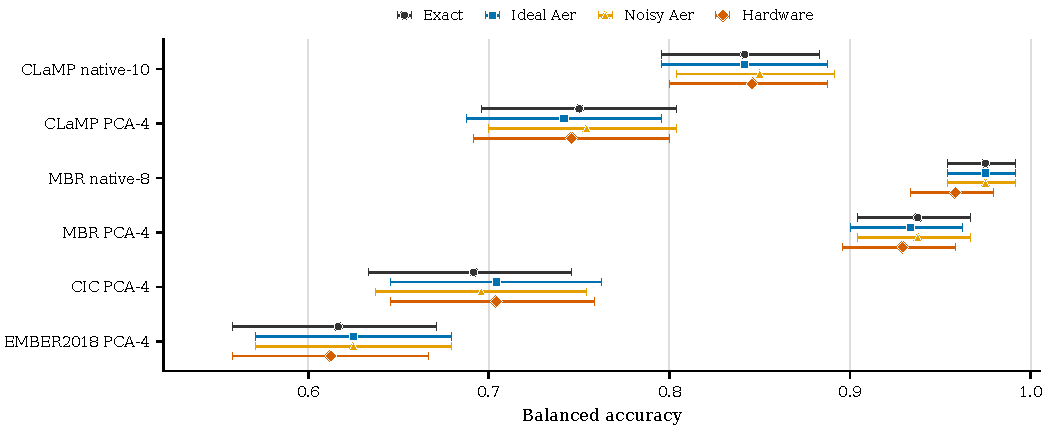
\includegraphics[width=\textwidth]{hardware_results/results/analysis/paper_figure1_execution_performance.pdf}
  \caption{Balanced accuracy across exact, ideal-Aer, noisy-Aer, and IBM hardware execution. Points are means across three held-out splits; bars are 95\% class-stratified bootstrap intervals based on 10,000 replicates and 240 held-out predictions per configuration and environment.}
  \label{fig:execution-performance}
\end{figure*}

The exact-to-ideal and ideal-to-noisy transitions likewise produced small balanced-accuracy changes. Across all configurations, exact balanced accuracy ranged from 0.617 to 0.975, ideal-Aer accuracy from 0.625 to 0.975, noisy-Aer accuracy from 0.625 to 0.975, and hardware accuracy from 0.613 to 0.958. Hardware ROC AUC ranged from 0.723 to 0.980. The two hardware measurements of each split-zero anchor yielded balanced-accuracy standard deviations of 0.009 at 4 qubits, 0.044 at 8 qubits, and 0.009 at 10 qubits.

\subsection{Kernel Distortion and Circuit Cost}

Kernel values changed monotonically with the execution ladder even when classification changed little (Figure~\ref{fig:kernel-distortion}). Ideal-Aer mean relative error ranged from 0.029 to 0.044. Noisy-Aer error ranged from 0.069 for EMBER2018 PCA-4 to 0.277 for CLaMP native-10. Hardware error clustered between 0.111 and 0.114 for all four-qubit configurations, compared with 0.441 for MBR native-8 and 0.479 for CLaMP native-10. Hardware kernel correlations with the exact kernel were 0.996--0.997 at four qubits, 0.924 at eight qubits, and 0.970 at ten qubits.

\begin{figure*}[t]
  \centering
  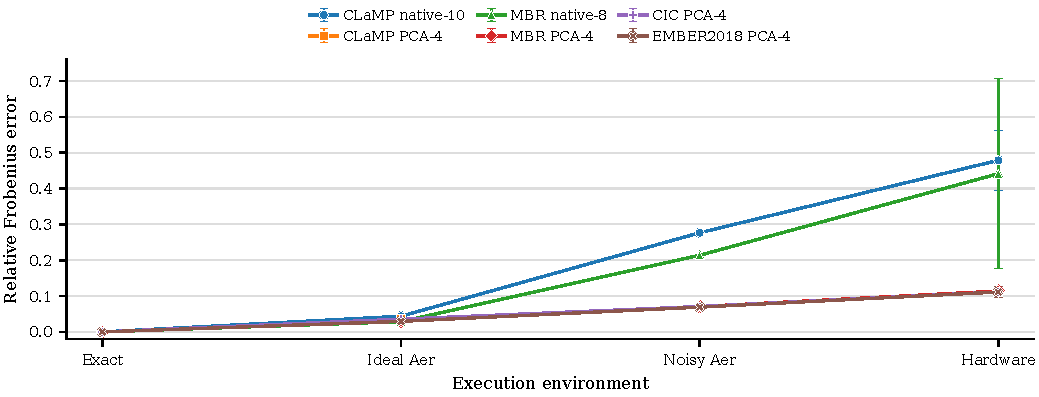
\includegraphics[width=\textwidth]{hardware_results/results/analysis/paper_figure2_kernel_distortion.pdf}
  \caption{Test-kernel relative Frobenius error against the exact statevector kernel. Markers are three-split means and error bars are split standard deviations. Exact kernels define the zero-error reference.}
  \label{fig:kernel-distortion}
\end{figure*}

Across the 18 primary hardware runs, CZ count had a descriptive Pearson correlation of 0.857 (Spearman $\rho=0.812$) with test-kernel relative error and $-0.032$ (Spearman $\rho=-0.129$) with hardware-minus-exact balanced accuracy (Figure~\ref{fig:circuit-cost}). These repeated-width associations are confounded by dataset and representation. Reducing CLaMP from native-10 to PCA-4 reduced depth from 206 to 98 and CZ count from 70 to 22, while hardware balanced accuracy decreased by 10.0 points. Exact CLaMP accuracy decreased by 9.2 points. The paired CLaMP hardware predictions favored native-10 over PCA-4 after Holm adjustment ($p=0.0179$). For MBR, PCA reduced width from eight to four qubits and CZ count from 54 to 22; hardware balanced accuracy decreased by 2.9 points, and the adjusted paired-test value was $p=0.458$.

\begin{figure*}[t]
  \centering
  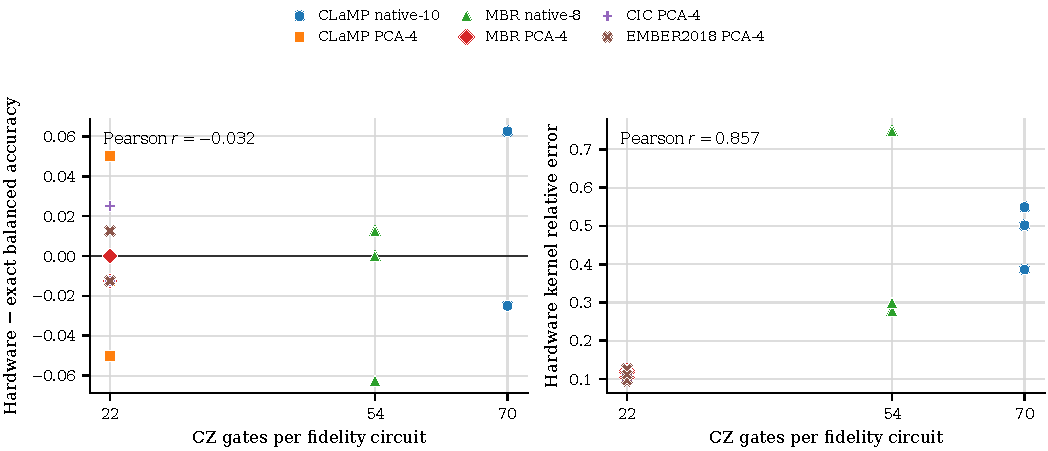
\includegraphics[width=0.98\textwidth]{hardware_results/results/analysis/paper_figure4_circuit_cost.pdf}
  \caption{Circuit cost, kernel distortion, and predictive change for the 18 primary hardware runs. Each point is one held-out split; CZ count is the transpiled two-qubit gate count per fidelity circuit. Correlations are descriptive because widths are not independently randomized across datasets.}
  \label{fig:circuit-cost}
\end{figure*}

The 21 hardware conditions totaled 200,760 kernel evaluations, 102,789,120 shots, and 28,189 seconds of IBM-reported QPU usage. Median QPU usage per 9,560-evaluation condition was 1,337 seconds at four qubits, 1,348 seconds at eight qubits, and 1,354 seconds at ten qubits. Linear projections from these measured condition totals give 58.3--59.0 QPU hours for a 1,000-training/1,000-test kernel workload and 679.7--688.4 hours for 5,000 training and 1,000 test observations; these are extrapolations rather than measured runs.

\subsection{Comparison with Classical Kernels}

Figure~\ref{fig:quantum-classical} reports matched classical checks. The RBF SVC mean balanced accuracies were 0.854, 0.754, 0.917, 0.921, 0.708, and 0.675 in configuration order. Corresponding hardware-quantum values were 0.846, 0.746, 0.958, 0.929, 0.704, and 0.613. Hardware-minus-RBF differences were therefore $-0.8$, $-0.8$, $+4.2$, $+0.8$, $-0.4$, and $-6.3$ percentage points. The linear SVC was lower than both nonlinear kernels in five configurations; on EMBER2018 its 0.621 mean was slightly above the 0.613 hardware result. These baseline comparisons were descriptive and were not included among the prespecified paired tests.

\begin{figure*}[t]
  \centering
  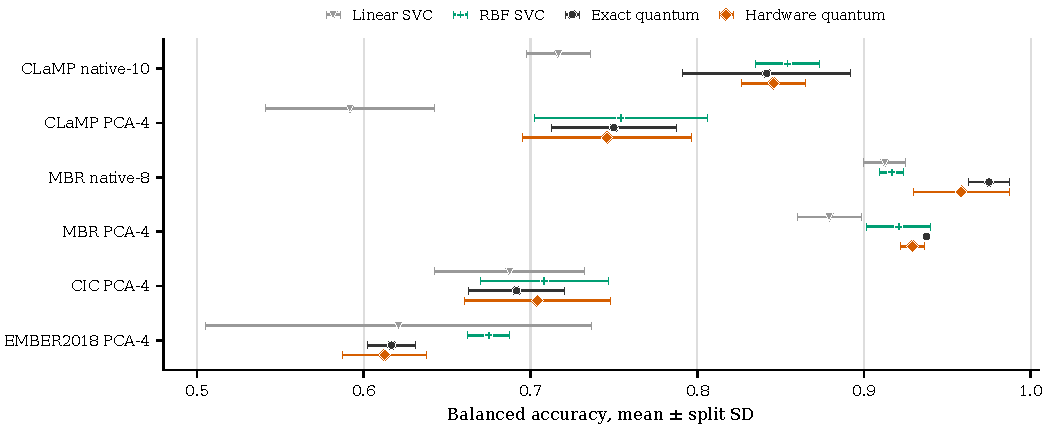
\includegraphics[width=\textwidth]{hardware_results/results/analysis/paper_figure3_quantum_classical.pdf}
  \caption{Matched linear-SVC, RBF-SVC, exact-quantum, and hardware-quantum balanced accuracy. Points are three-split means and bars are split standard deviations. Every classifier used $C=1$ without hyperparameter tuning.}
  \label{fig:quantum-classical}
\end{figure*}

\section{Discussion and Conclusion}

The measured IBM kernels preserved balanced accuracy across all six configurations despite greater numerical distortion than exact and Aer kernels. Hardware-minus-exact changes remained within $-1.67$ to $+1.25$ percentage points, and none was significant under the prespecified Holm-adjusted paired analysis. This result establishes empirical stability for the tested samples, feature map, classifier, shot budget, backend, and calibration window. It does not establish statistical equivalence between hardware and exact execution.

Feature compression reduced circuit width, depth, two-qubit gates, and hardware kernel distortion. Its predictive effect was dataset dependent. CLaMP PCA-4 reduced hardware balanced accuracy by 10.0 points relative to native-10, whereas MBR PCA-4 reduced it by 2.9 points relative to native-8. The difference-in-differences estimates for whether compression altered hardware degradation itself were $-0.8$ points for CLaMP and $+0.8$ points for MBR, with wide descriptive three-split intervals spanning zero. The observed accuracy loss was therefore associated primarily with the compressed representation rather than an identified compression-by-hardware interaction.

The classical checks do not support a consistent predictive quantum advantage. RBF balanced accuracy matched or exceeded hardware quantum accuracy on both CLaMP configurations, CIC, and EMBER2018; the hardware quantum kernel was descriptively higher on both MBR configurations. No method was tuned, the training sets contained only 80 observations, and no paired quantum-versus-classical hypothesis tests were prespecified. The experiment also recorded neither end-to-end comparable wall-clock time nor system-level energy use. It consequently provides no evidence of speed or energy advantage. The quadratic kernel workload and measured QPU-time projections further limit direct scaling of the present protocol.

Several constraints bound the findings. Balanced 80/80 splits do not reproduce operational malware prevalence, and three repeated holdouts provide limited information about sampling variation. The four datasets differ in collection process and observation unit: three describe PE files, whereas CIC describes sandbox activity records. The study tested one feature map, one entanglement pattern, one repetition count, one shot count, fixed $C=1$, one device, one transpilation, and one primary calibration window. Error mitigation was intentionally disabled, and the classical comparison was not a tuned benchmark. Width, dataset, and representation were coupled, so the circuit-cost correlations are descriptive rather than causal. The bootstrap intervals condition on sampled rows and preprocessing choices, while the three-split compression intervals are imprecise.

Splits were disjoint by source-row identifier and by the full numeric vector used by each model. A post hoc audit of the CIC metadata found that two file hashes recurred across different held-out splits, although no hash appeared in both training and test data within any evaluated split. CIC therefore does not support file-independent inference across pooled splits. Future evaluations should group CIC observations by binary hash and sandbox session, and should use family-aware or temporal holdouts. The MBR analysis also depends on the specific Kaggle file version and its upstream sample provenance. None of the reported values should be interpreted as full-corpus detector performance or performance under novel malware-family distribution shift.

Under these conditions, four-qubit PCA kernels showed low hardware distortion, while wider kernels showed substantially larger distortion without corresponding loss of balanced accuracy. The practical result is a reproducible demonstration of hardware robustness in a small-sample malware-classification workflow, coupled with a measurable representation--resource tradeoff. Establishing quantum advantage will require larger group-disjoint and temporal evaluations, nested tuning of classical and quantum models, repeated executions across devices and calibrations, explicit mitigation ablations, and comparable measurements of latency and energy.
